\documentclass[11pt, a4paper, twocolumn]{article}

\usepackage{tikz}
\usepackage{tikz,fullpage}
\usetikzlibrary{arrows,%
	petri,%
	topaths}%
\usepackage{tkz-berge}
\usepackage{amsmath}
\usepackage{amsfonts}
\usepackage{amssymb}

\usepackage{textcomp}
\usepackage{logicproof}
\usepackage{float}
\usepackage{hyperref}
\usepackage[T1]{fontenc}
\usepackage[]{algorithm2e}
\usepackage{parskip}
\usepackage[toc,page]{appendix}
\usepackage{graphicx}
\usepackage{subcaption}
\usepackage[lmargin=0.3in,rmargin=0.3in,tmargin=0.3in,bmargin=0.6in]{geometry}
\graphicspath{  {../Saved_Figs/} {../Dataset/} }
%opening
\title{\vspace{-1.25cm}Machine Learning Coursework - OULAD Analysis}
\author{mbtj48}
\date{}

\begin{document}

\maketitle

\section{Data Gathering \& Analysis}

Machine learning \& data gathering are paramount for modern, cutting edge technologies; thus we have been tasked to develop 2 machine learning models to predict final grades from the OULAD.

\begin{figure}[H]
	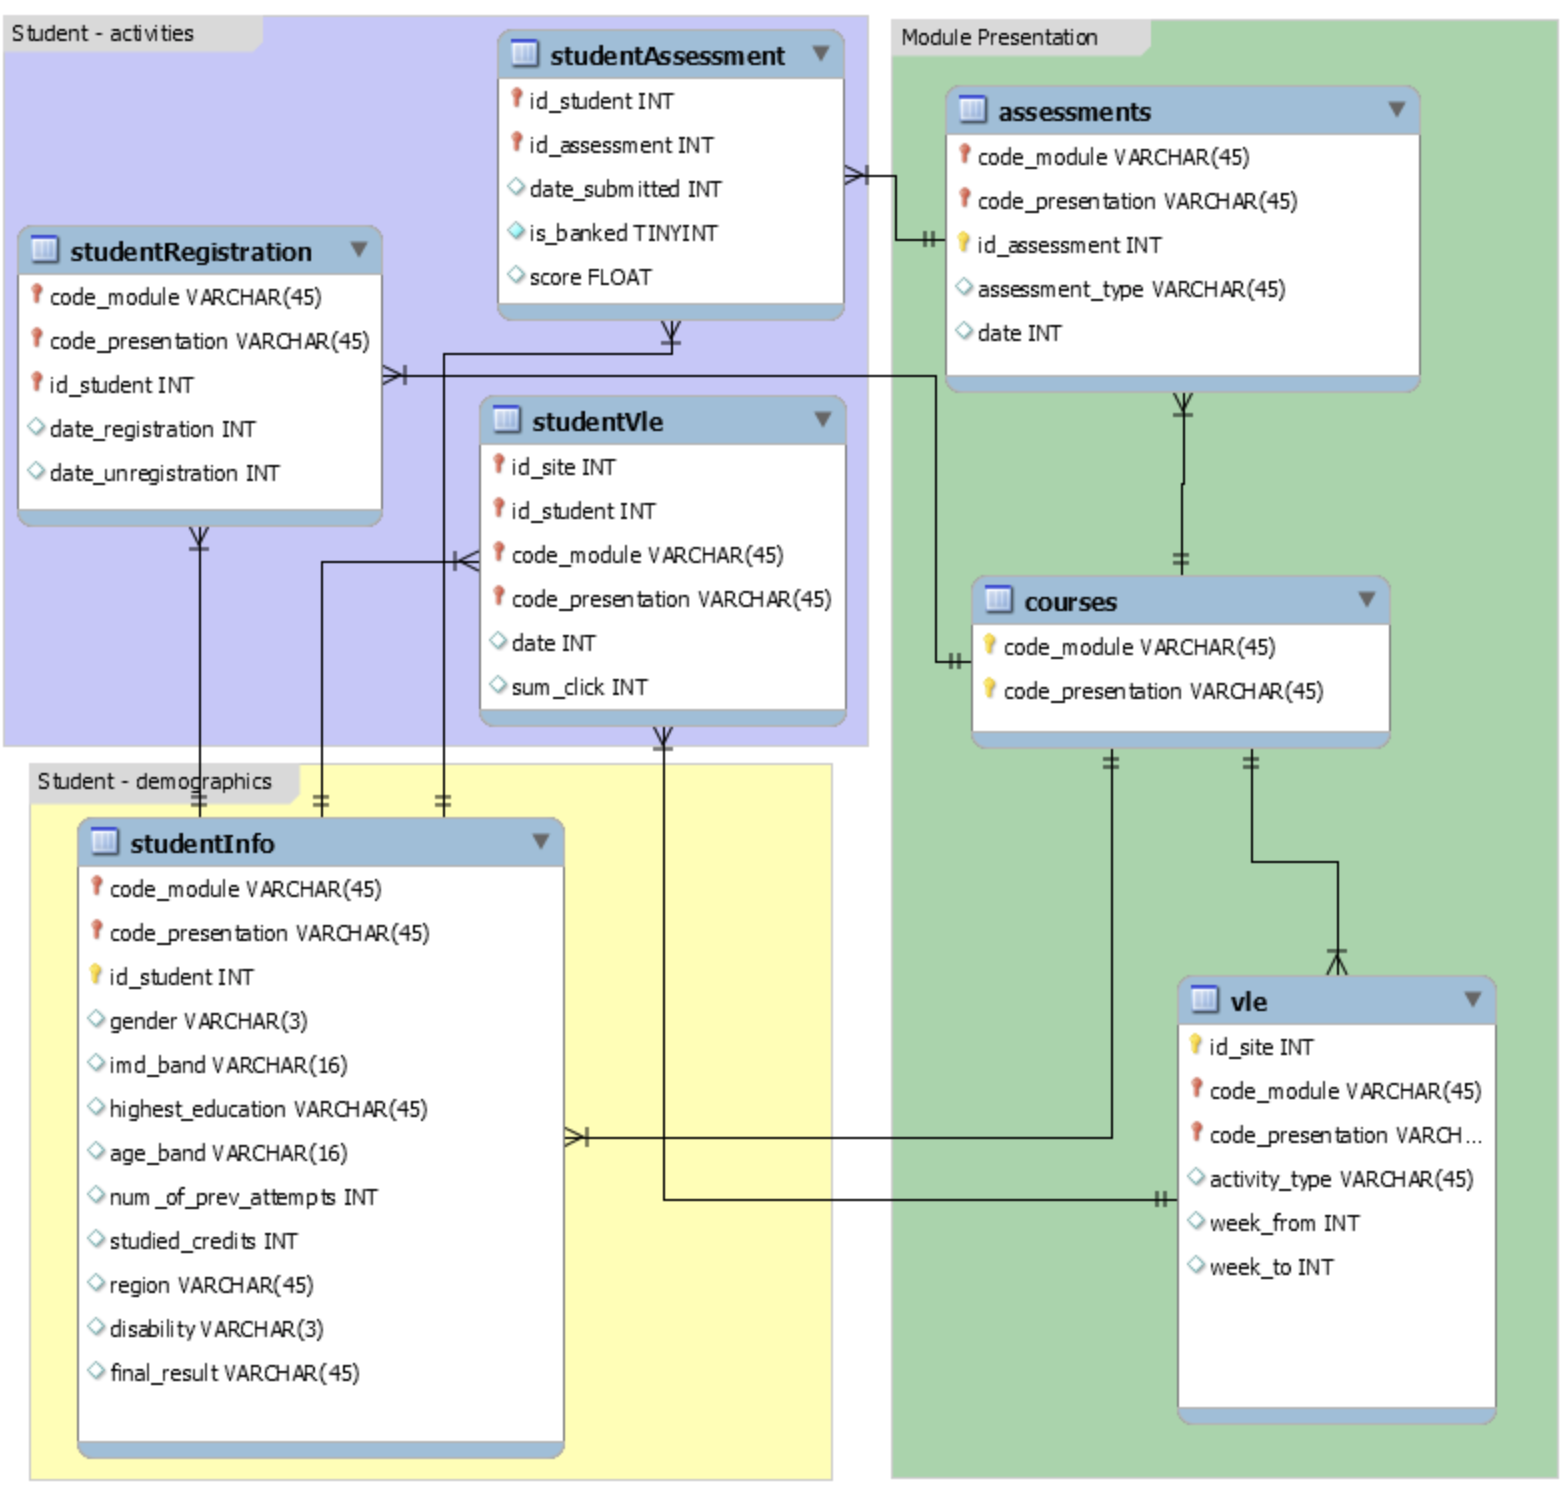
\includegraphics[width=\linewidth]{dataset.png} 
	\caption{Dataset Schema}
	\label{fig:schema}
\end{figure}

Firstly, I noticed useful features such as the score in the studentAssessment table, \& sum\_click in the studentVle table.
Therefore I started by grouping the sum\_click and score features, finding the net clicks within the portal for a given student through the year \& their average mark. 
I expected these features to show a positive correlation because typically higher scores and grades may come from more effort which is implied by the portal visits. N.b. This is shown in \ref{table:heatmap}.
Then, I plotted the data and noticed that a logistic regression model should perform highly. 
I added more data to my model, to use as much data as possible so the model can find patterns easier.
Further, I calculated how many days early a student submitted coursework using the date submitted column.
Ideally, I expected a positive correlation as the student would be more prepared and commited.
In addition, I calculated their summative and formative (where their weight is 0) marks. 
% I noticed this gradually improved the performance of my model, so I continued adding further data.
I eventually included almost all of the data available, so I started to look at the data differently so I included the mean, mean absolute deviation, standard deviation, varience etc for the scores of students' coursework.
This therefore can find patterns from extrapolated data to squeeze more patterns out of the schema. 
I then produced a correlation heatmap as seen below, as well as the sorted numerical correlations.


\begin{table}[H]
	\centering
	\begin{tabular}{|l|l|}
		\hline
		Feature                    & Correlation \\ \hline
		daysEarlystdScore            & $-0.259014$ \\ \hline
		studied\_credits             & $-0.176016$ \\ \hline
		region\_Wales                & $0.008382$  \\ \hline
		age\_band                    & $0.068551$  \\ \hline
		score                        & $0.317339$  \\ \hline
		sum\_click                   & $0.376107$  \\ \hline
		totalCoursework              & $0.427175$  \\ \hline
		summativeAgainstCredits      & $0.490646$  \\ \hline
		\end{tabular}
		\caption{Correlations}
		\label{table:Correlations}
\end{table}

Surprisingly, age\_band has a poor correlation, in theory you would expect a mild negative correlation. Although this could be because of the limited data (3 unique ranges). To improve this correlation, I would need specific precise data.


After data gathering, I preprocessed the data, with an imputer and scaler. The imputer changes all NA values to the median of that feature. 
While the scaler, normalises features to be within $0-1$, this prevents feature domination with large ranges and makes the features unit dependent
Further, I exchanged region, code module and code presentation to columned data by one hot encoding those categories.

\section{Model Selection}

The following phase was selecting a model. Here, I split the data into train and test sets with a 75/25 split; then tested a variety of models and compared how they performed in cross validation on the training data.



\section{Model A - Logistic Regression}

After I picked logistic regression, I began my hyperparameter tuning. For this model, I decided to use a grid search to validate the best parameter within the permutations I provided. 
I gave the model, two potential sets of permutations, the first, cycled through the C value, which is the regularisation strength; smaller values show a stronger strength, 
so I started with a strong logarithmic scale to check through, until after enough testing I used the range between 950 and 1125. It also cycled through the tolerance value with small values around the default of 0.0001.
The other set of permutations loop through a similar set of values of C and adjusts the max number of iterations model uses to fit the data and find patterns.

\section{Model B - Random Forest Regressor}

Following my logistic hyperparameter tuning, I tuned my random forrest regressor, using a random search. This randomly picks n permutations to validate the model against based on the given parameters.
I decided to check the number of estimators (trees in forrest), the max depth of each tree in the forrest, the minimum number of samples required at a leaf node, \& the minimum number of samples required to split an internal node.
As the random search prefers ranges, all of these values are provided with the python range type so it can pick any value within the range. This lead to picking 20 out of 244,800 permutations of parameters.

\section{Conclusion}

\begin{table}[H]
	\centering
	\begin{tabular}{l|l|l|}
	\cline{2-3}
												   & Logistic & Random Forrest \\ \hline
	\multicolumn{1}{|l|}{Explained Var} 		   & 0.361                     & 0.604                           \\ \hline
	\multicolumn{1}{|l|}{Mean Abs Err}       	   & 0.393                     & 0.405                           \\ \hline
	\multicolumn{1}{|l|}{Mean Square Err}          & 0.513                     & 0.309                           \\ \hline
	\multicolumn{1}{|l|}{RMSE}   				   & 0.716                     & 0.556                           \\ \hline
	\multicolumn{1}{|l|}{Med Abs Err}    		   & 0.000                     & 0.318                           \\ \hline
	\multicolumn{1}{|l|}{r2 Score}                 & 0.343                     & 0.604                           \\ \hline
	\multicolumn{1}{|l|}{Best Score}               & 0.678                     & 0.590                           \\ \hline
	\end{tabular}
	\caption{Metrics of Final Models}
	\label{table:metrics}
\end{table}

In conclusion, the logistic regression model finished with an accuracy of 0.68\%, whereas the Random Forrest Model finished with an accuracy of 0.59\%, therefore making the logistic model initially more desirable.
Upon further inspection and validation on the testing data set, the maxiumum error was 0.3 lower for the random forrest, \& the r2 score was 0.25 higher for random forrest, potentially making random forrest overall a better choice.

\section*{Appendix}
\centering
% \begin{figure}[H]
% 	\includegraphics[width=0.95\linewidth]{age_band_linear_model.png} 
% 	\caption{Age band against Final Result Linear Regression Model}
% 	\label{fig:AgeLin}
% \end{figure}
% \centering
% \begin{figure}[H]
% 	\includegraphics[width=0.95\linewidth]{sum_click_SVR_linear_model.png} 
% 	\caption{Total VLE clicks against Final Result SVR (Linear Kernel) Regression Model}
% 	\label{fig:clickSVRLin}
% \end{figure}
% \centering
% \begin{figure}[H]
% 	\includegraphics[width=0.95\linewidth]{score_linear_model.png} 
% 	\caption{Score against Final Result Linear Regression Model}
% 	\label{fig:scoreLinear}
% \end{figure}



% \begin{figure}[H]
% 	\includegraphics[width=\linewidth]{score_linear_model.png} 
% 	\caption{Score against Final Result Linear Regression Model}
% 	\label{fig:scoreLinear}
% \end{figure}
	
\end{document}
